\documentclass[english]{beamer}
\usepackage[english]{babel}
\usepackage[utf8]{inputenx}
\usepackage[T1]{fontenc}      % Font encoding
\usepackage{lmodern}          % lmodern font, correctly copyable characters in pdf

\usepackage{hyperref}
\usepackage{bookmark}
\usepackage{soul}
\newcommand{\code}[1]{\texttt{#1}}

\usetheme[
  bullet=circle,                  % Use circles instead of squares for bullets
  titleline=false,                % Show a line below the frame
  alternativetitlepage=true,      % Use the fancy title
  titlepagelogo=logo-sapienza,    % Logo for the first slide
  watermark=watermark-diag,   % Watermark used in every slide
  watermarkheight=20px,           % Desired height of the watermark
  watermarkheightmult=6,          % Watermark image is actually x times bigger
  displayauthoronfooter=true,     % Display author name in the footer
]{Roma}
\watermarkoff
\author{G07: \underline{Dario Loi}, Davide Marincione}
\title{Predicting player's movements in CSGO}
\subtitle{Or how we \emph{forcefully} applied statistics on a competitive FPS}
\institute{Bachelor's degree in\\Applied Computer Science and Artificial Intelligence\\Sapienza, University of Rome}
\date{A. Y. 2021 - 2022}

\begin{document}

\begin{frame}[t,plain]
\titlepage
\end{frame}

\section{What?}
\begin{frame}{The hell's a "CSGO"?}
  \begin{figure}
    \centering
      
\includegraphics[width=.7\textwidth]{images/csgo_alt.png}
      \caption{CSGO's logo.}
  \end{figure}
\end{frame}

\section{Why?}
\begin{frame}{Why did you do this?}
  We had our reasons for this choice (of course), some of those being:

  \begin{columns}
    \begin{column}{0.49\textwidth}
      \begin{itemize}
        \item Videogames offer wide data availability.
        \item Prediction of an erratic phenomena such as movement is impressive \emph{if done right}.
      \end{itemize}
    \end{column}

    \begin{column}{0.49\textwidth}
      \begin{itemize}
        \item The process of collecting data with the collaboration of our colleagues was very appealing\footnotemark[1].
        \item It \emph{seemed} like fun.
      \end{itemize}
      
    \end{column}
  \end{columns}
  \footnotetext[1]{You don't get to play games for university \emph{that} often.}
\end{frame}

\section{Giving structure}

\begin{frame}{The Game Map}
  \begin{columns}
    \begin{column}{0.55\textwidth}
    The choice for our environment immediately fell on the popular map \code{de\_dust2}, both because we are highly familiar with it and `cause it is,
    by a large margin, the most played map of the game, meaning that eventual test subjects would be familiar with playing it and, in the worst case\footnotemark[2]
    there would be available data from outside sources.
    \end{column}
    \begin{column}{0.45\textwidth}
      \begin{figure}
      \centering
      \includegraphics[width=1\textwidth]{images/Dust2\_asite1.jpg}
      \caption{A \emph{beautiful} shot of Dust2's A site\dots}
      \end{figure}
    \end{column}
  \end{columns}

  \footnotetext[2]{which did present itself, as we were forced to make use of competitive matches for data due to time constraints.}
\end{frame}

\begin{frame}{Hexagons are the best-a-gons}
  In order to properly process the game data and capture it in a statistical framework, we had to abstract the map's geometry into some neat 
  geometrical primitives, the natural solution would be tiling the map with squares, but the best one turns out to be \emph{hexagons}:

  \begin{columns}
    \begin{column}{0.5\textwidth}
      \begin{itemize}
        \item Definition of \emph{neighbour} is unambiguous.
        \item Distance between two hexagons' centers is \emph{constant}.
      \end{itemize}
    \end{column}
    \begin{column}{0.5\textwidth}
      \begin{itemize}
        \item More sides, leading to finer granularity of movement.
        \item Best approximation of a circle capable of tiling a plane.
        \item Looks Fancy.\footnotemark[3]
      \end{itemize}
    \end{column}
  \end{columns}
  \footnotetext[3]{And reminds us of strategy games.}
\end{frame}

\begin{frame}{Heuristics shenanigans}
  \begin{columns}
    \begin{column}{0.5\textwidth}
      In the discretization of the map we faced two problems:
      \begin{itemize}
        \item Extrapolating height data.
        \item Create hexagons (cells) for areas of the map that do overlap each other.
      \end{itemize}
      For both cases we used heuristics\footnote{We describe them in the documentation.} and a bit of eyeballing.
    \end{column}
    \begin{column}{0.5\textwidth}
      \begin{figure}[h]
        \centering
        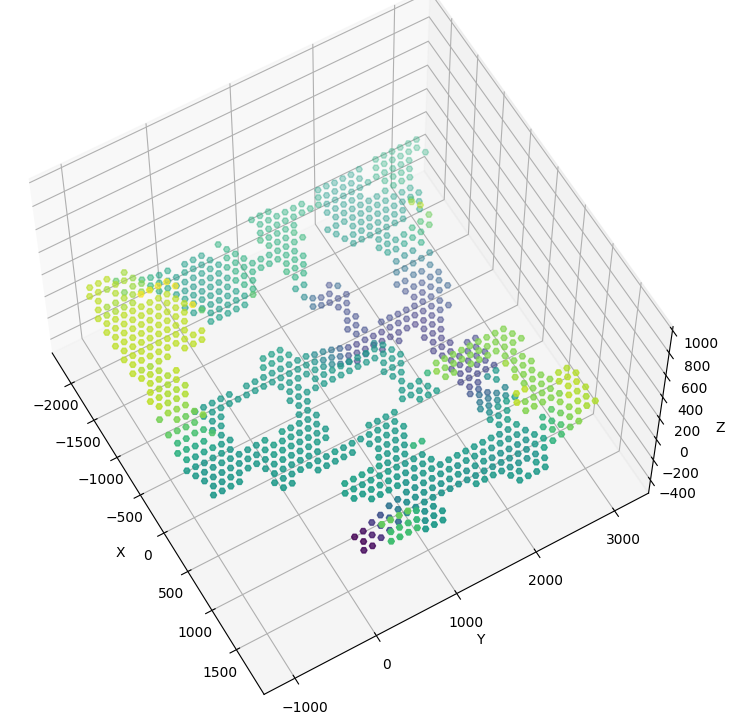
\includegraphics[width=0.85\textwidth]{images/post_tiling2.png}
        \caption{Our final tiling}
      \end{figure}
    \end{column}
  \end{columns}
\end{frame}

\begin{frame}{A graph\dots Markov Chains?!}
  \begin{columns}
    \begin{column}{0.55\textwidth}
      At the end of our tiling process, we had obtained a directed graph that represented our map\footnote{It is here that we realized that Markov Chains would be a proper statistical tool, but too little too late.}, in it, we utilized 
      symmetrical (undirected) edges for \emph{walkable} connections and directed edges for places with a different height, in which 
      it is possible to jump down but not to climb up.

    \end{column}
    \begin{column}{0.45\textwidth}
      \begin{figure}
        \centering
        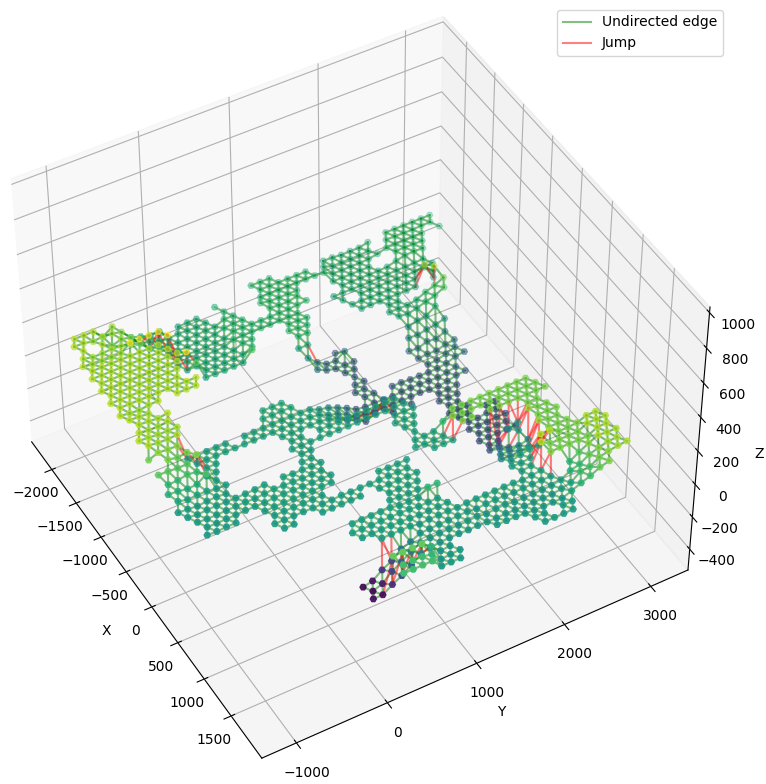
\includegraphics[width=1\textwidth]{images/graph.png}
        \caption{Dust2's graph, showing edges between our tiles.}
        \end{figure}
    \end{column}
  \end{columns}

\end{frame}


\begin{frame}{Nearsightedness problems}
  \begin{columns}
    \begin{column}{0.55\textwidth}
      Another information we wanted to provide (that we \emph{hoped} to use) was of the line of sight available to a player, and thus whether one was able, during a frame, to see another... it was a \emph{bit} problematic.
    \end{column}
    \begin{column}{0.45\textwidth}
      \begin{figure}
        \centering
        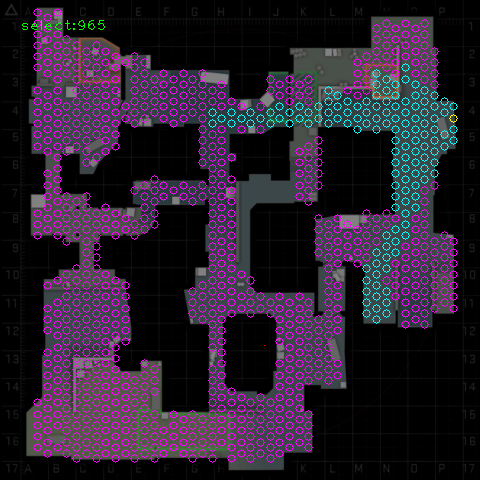
\includegraphics[width=1\textwidth]{images/view_car.png}
        \caption{Painstakingly hand-made line-of-sight info, for \emph{one} cell.}
        \end{figure}
    \end{column}
  \end{columns}
\end{frame}

\section{Our theory}
\begin{frame}{A single step}

  From the current cell, propose the distribution of the next possible position based on some current information/action.

  \begin{figure}
    \centering
    \begin{equation*}
      \mathbf{E}\left( \mathbf{P}\left(K_2\right) | K_0 \to K_1\right) =
      \begin{cases}
          \mathbf{P}\left(K_2 = K_1\right)\\
          \mathbf{P}\left(K_2 = A\right)\\
          \mathbf{P}\left(K_2 = B\right)\\
          \dots
      \end{cases}
    \end{equation*}
    \caption{Example of the expected distribution for the next position, given the last movement.}
  \end{figure}
\end{frame}

\begin{frame}{Inductive process!}
  Using (abusing) the law of total expectation, we can derive not only the very next position, but also the ones after that!

  \begin{align*}
  &\mathbf{E}\left( \mathbf{P}\left(K_3\right) | K_0 \to K_1\right) =\\
  \sum_{n \in N_{K_1}} &\mathbf{E}\left( \mathbf{P}\left(K_3\right)  | K_1 \to n\right)\cdot\mathbf{E}\left(\mathrm{P}(K_2 = n) | K_0 \to K_1\right)
  \end{align*}

  This may continue for any depth!
\end{frame}

\section{Data collection}
\begin{frame}{Our unused idea}
  \begin{columns}
    \begin{column}{0.55\textwidth}
      One of our main motivations for the project was the possibility of course mate engagement in the sampling process, for this purpose, we built a small plug-in capable of managing 
      the game's flow according to our experiment.
      
      Unfortunately, time was running out and nobody seemed available for such an activity, so we had to scrap this and gather the data 
      from popular competitive website \href{https://www.hltv.org/}{HLTV}.
    \end{column}
    \begin{column}{0.45\textwidth}
      \begin{figure}
        \centering
        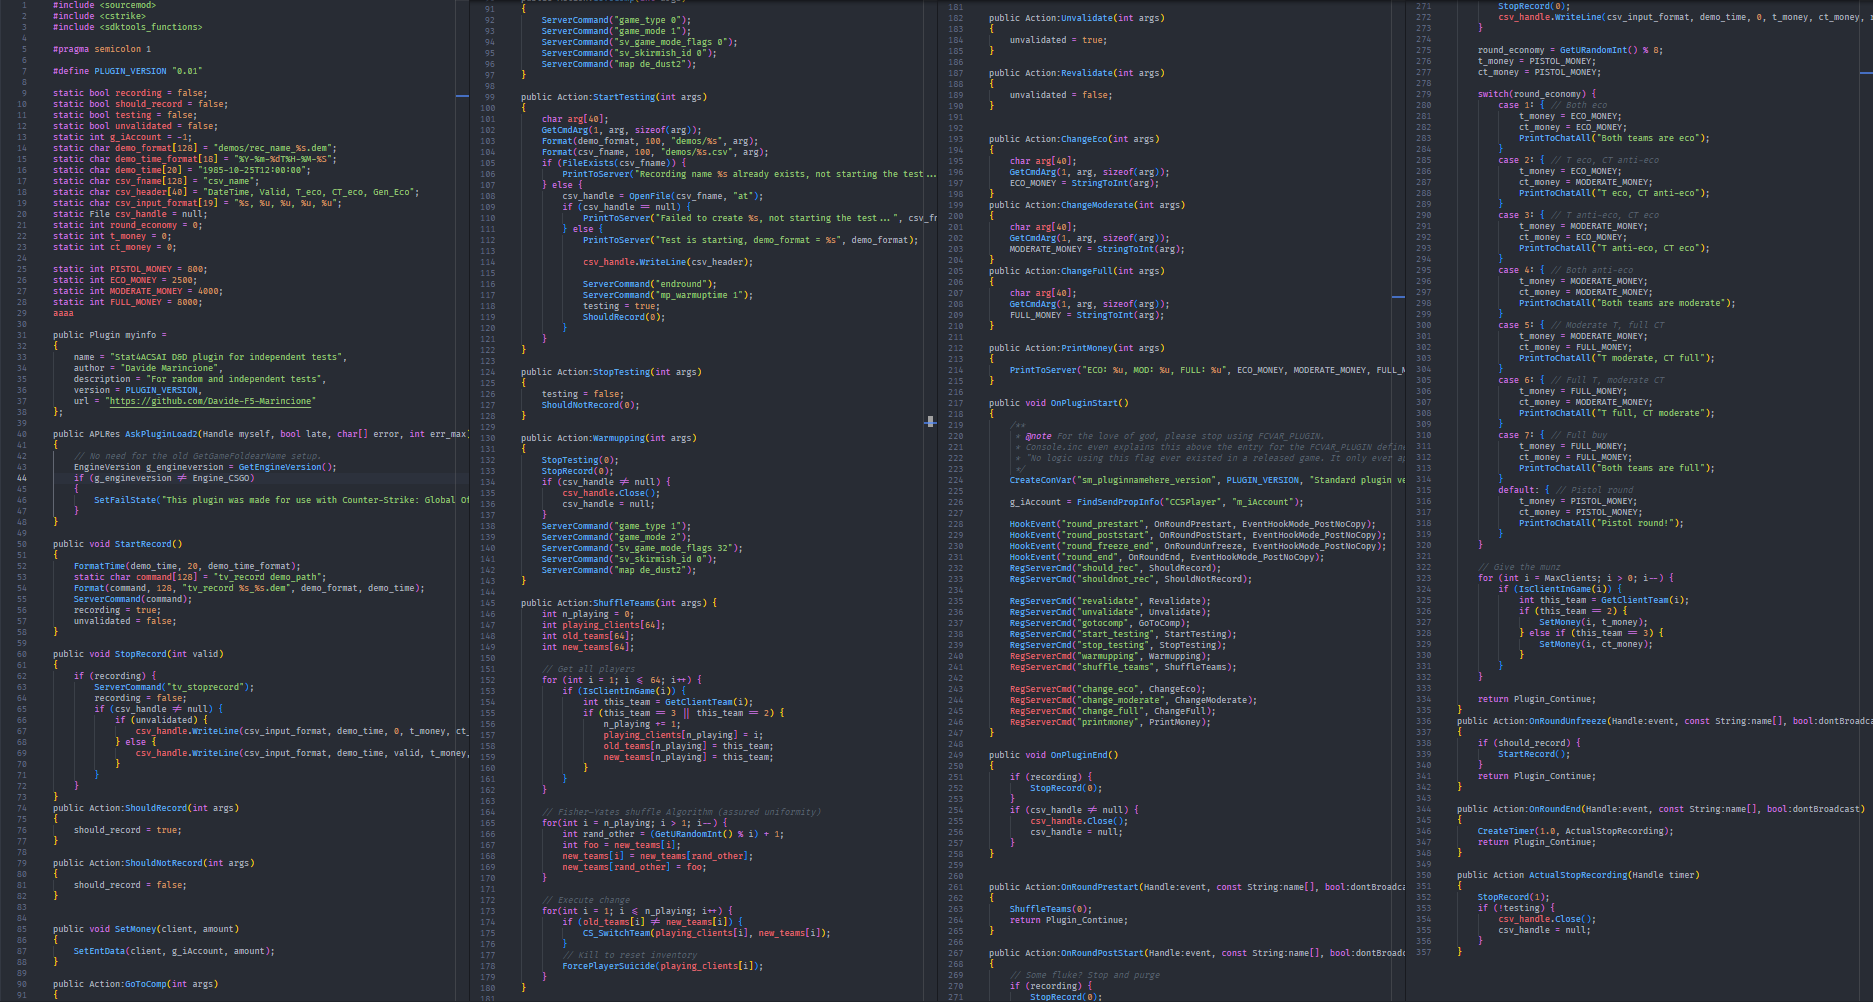
\includegraphics[width=1\textwidth]{images/plugin_code.png}
        \caption{Our useless plugin, \emph{squeezed} into a single image}
        \end{figure}
    \end{column}
  \end{columns}
\end{frame}

\begin{frame}{Extraction and cleaning}
  \begin{columns}
    \begin{column}{0.55\textwidth}
      A sample is composed of:
      \begin{itemize}
        \item Next movement (response var).
        \item Player's team.
        \item Previous movement.
        \item Team's center of mass orientation (useless).
        \item Number of teammates (useless).
      \end{itemize}
     The number of training samples in the end was around 540'000, while the test set amounted to 390'000.
    \end{column}
    \begin{column}{0.45\textwidth}
      \begin{figure}
        \centering
        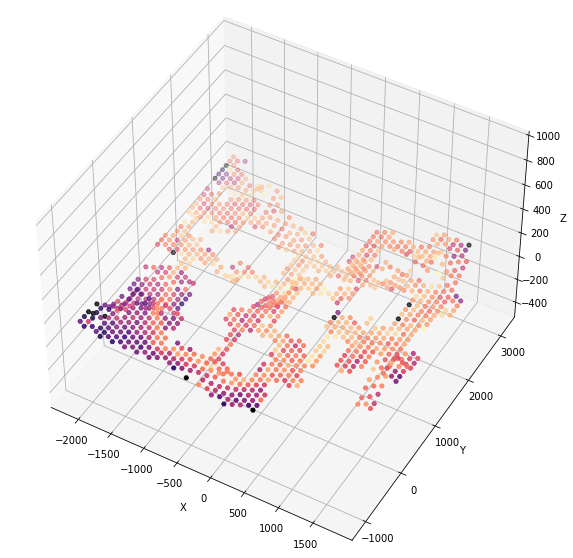
\includegraphics[width=1\textwidth]{images/samples_count.png}
        \caption{Overall distribution of our training set}
      \end{figure}
    \end{column}
  \end{columns}
\end{frame}

\section{The predictor}
\begin{frame}{Bagging! Sorta\dots}

  \begin{columns}
    \begin{column}{0.5\textwidth}
      To regress a model for each cell we need enough data\dots Unfortunately in some cases this luxury wasn't available: thus we made multiple models of different quality.
    \end{column}
    \begin{column}{0.5\textwidth}
      \begin{enumerate}
        \item \texttt{choice \raisebox{-0.3ex}{\textasciitilde} 1}
        \item \texttt{choice \raisebox{-0.3ex}{\textasciitilde} team}
        \item \texttt{choice \raisebox{-0.3ex}{\textasciitilde} cell\_from}
        \item \texttt{choice \raisebox{-0.3ex}{\textasciitilde} cell\_from * team}
        \item \texttt{choice \raisebox{-0.3ex}{\textasciitilde} cell\_from * team + dir\_team}
      \end{enumerate}
    \end{column}
  \end{columns}

  \begin{center}
    \begin{tabular} {l c c c}
        Model\# & Cells present & $\overline{\rho}^2$ (present) & $\overline{\rho}^2_a$ (present)\\
        \hline
        1 & 43 & $0.00$ & $0.00$\\
        2 & 161 & $0.11$ & $0.01$\\
        3 & 264 & $0.25$ & $0.22$\\
        4 & 477 & $0.23$ & $0.20$\\
        \hline
        Tot & 945 & $0.20$ & $0.17$
    \end{tabular}
  \end{center}
\end{frame}

\begin{frame}{The algorithm}
  \begin{columns}
    \begin{column}{0.55\textwidth}
      Our theory may take a \emph{lot} to run if written in a naive way, roughly $O(7^d)$. That's why our algorithm approximates it through two tricks:

      \begin{itemize}
        \item A cut-off.
        \item Memoization.
      \end{itemize}
    \end{column}
    \begin{column}{0.45\textwidth}
      \begin{figure}
        \centering
        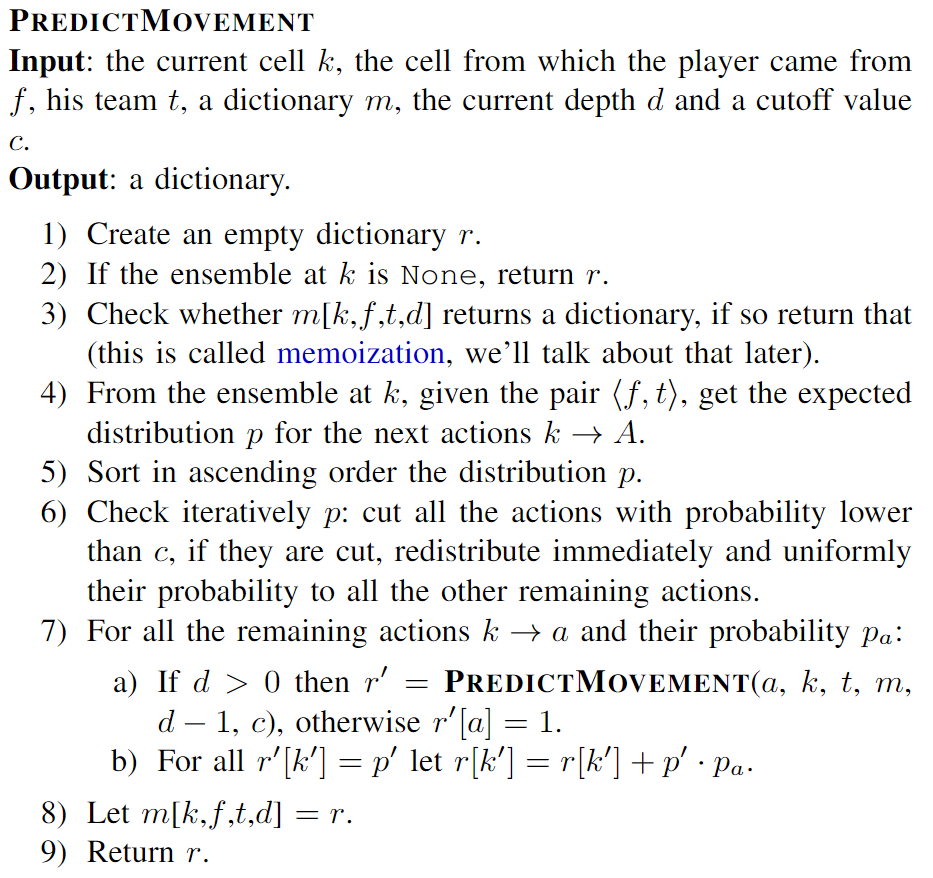
\includegraphics[width=1\textwidth]{images/pseudo_code.png}
        \caption{Pseudo-code!}
      \end{figure}
    \end{column}
  \end{columns}

\end{frame}

\begin{frame}{A matter of opinions}
  \begin{columns}
    \begin{column}{0.45\textwidth}
      Our model outputs a distribution of the probabilities of presence of a player in a range of given hexagons, in order to tailor the way that 
      this distribution is presented, we propose an hyperparameter, \emph{accumulation} ($\gamma$), which acts as a threshold for our tiles, allowing us to 
      present a more \emph{meaningful} distribution.
    \end{column}
    \begin{column}{0.55\textwidth}
      \begin{figure}
        \centering
        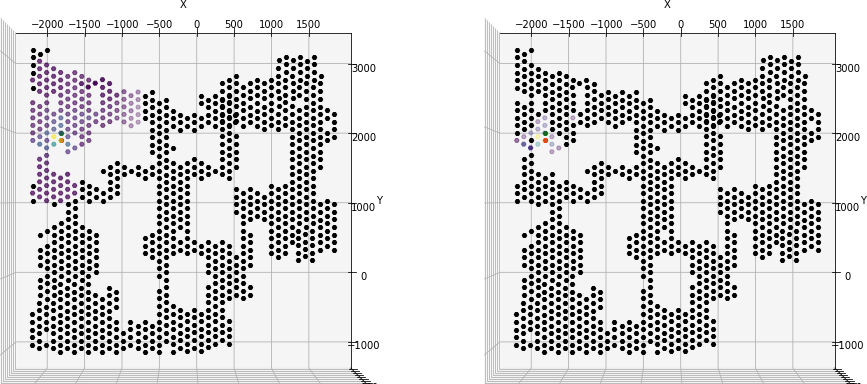
\includegraphics[width=1\textwidth]{images/wildfire_v_non2.png}
        \caption{To the left, one of our model's predictions, to the right, the same prediction that went through the accumulation process, $\gamma = 0.7$.}
        \end{figure}
    \end{column}
  \end{columns}
\end{frame}

\begin{frame}{Conclusions}
  We believe that, with this project we accomplished:
  \begin{itemize}
    \item A solid model for movement prediction.
    \item A good set of tools capable of parsing \emph{any} in game map in order to apply our model
    \item A much more solid understanding of Generalized Linear Models
  \end{itemize}
  Therefore, the aims were nothing short of satisfied, given that we both enriched our knowledge and presented a working solution.
\end{frame}

\end{document}